\section{Background}

Retail stores depend on in-store staff to manually inspect shelves, identify empty spaces, and restock products. This traditional workflow is costly, slow, and vulnerable to human error, which can lead to stockouts and missed sales opportunities. This is particularly critical for FMCG (Fast-Moving Consumer Goods) companies where product availability directly impacts sales and customer satisfaction.
\\
Modern retail operations increasingly require automated monitoring to deliver consistent availability, reduce shrinkage, and improve customer satisfaction. Camera-based shelf monitoring provides an opportunity to detect product occupancy in real time and surface restocking alerts before shelves become empty.

\section{Problem Statement}

\begin{itemize}
    \item Retail staff must physically walk through aisles to check shelf inventory, which is time-consuming and distracts from customer service.
    \item Manual inspection can miss low-stock conditions and lead to empty display areas that reduce sales and damage the store experience.
    \item Conventional inventory systems often rely on shipment and sales data instead of actual shelf presence, leaving a gap between stock records and physical availability.
    \item Small retail stores lack practical and affordable shelf monitoring systems compared to large supermarket chains.
\end{itemize}

\section{Proposed Solution}

This project proposes an \textbf{Automated Shelf Monitoring System} that uses computer vision to monitor product occupancy on retail shelves. The system uses YOLOv8 (a state-of-the-art object detection model) to analyze camera images, detect whether products are present or missing from shelf regions, and generate automatic alerts when restocking is needed.
\\
Key capabilities include:
\begin{itemize}
    \item Real-time detection of shelf occupancy using YOLOv8n (nano) - optimized for speed.
    \item Product and category recognition for common retail items.
    \item Alert generation for low-stock or empty shelf regions.
    \item A dashboard summary for store staff.
    \item Edge deployment capability for real-time processing without cloud dependency.
\end{itemize}

\section{Project Scope}

The project focuses on a pilot implementation suitable for convenience and grocery stores. It includes:
\begin{itemize}
    \item A vision model for shelf occupancy detection.
    \item A simple processing pipeline that converts camera frames into stock status.
    \item An alerting mechanism for restocking events.
    \item A compact evaluation on a representative dataset.
\end{itemize}

\begin{figure}[H]
    \centering
    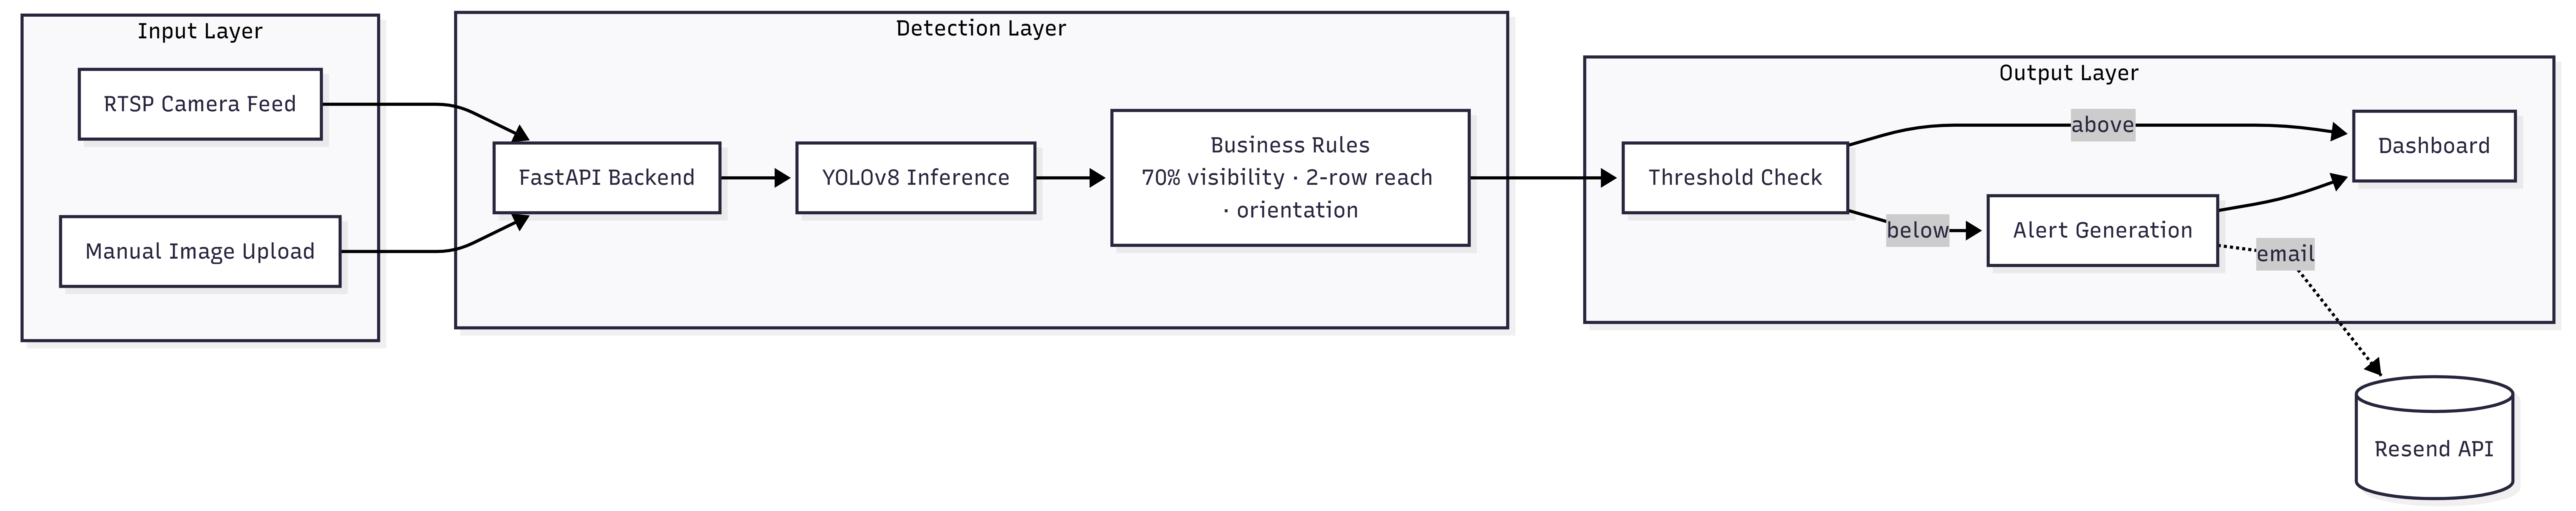
\includegraphics[width=0.8\textwidth]{figures/diagram_1.png}
    \caption{System Overview}
    \label{fig:system-overview}
\end{figure}

\section{Objectives}

The main objectives are:
\begin{enumerate}
    \item Develop a computer vision-based shelf monitoring prototype.
    \item Evaluate detection accuracy and shelf occupancy estimates.
    \item Demonstrate how alerts can support retail staff in reducing stockouts.
    \item Align the solution with Multinet's retail automation needs.
\end{enumerate}

\section{Report Structure}

This report is organized as follows:
\begin{itemize}
    \item Chapter 2 reviews related work in retail shelf monitoring and computer vision.
    \item Chapter 3 defines the software requirements and system constraints.
    \item Chapter 4 describes the system design and architectural decisions.
    \item Chapter 5 presents the implementation details, experiments, and evaluation results.
    \item Chapter 6 concludes the project and outlines future work.
    \item Chapter 7 provides a reflection on the project experience.
\end{itemize}
